We discuss the optimization opportunities and challenges through the following example of 3 queries (Query 3, 43 and 55) from the TPC-DS benchmark \cite{tpcds}:
\begingroup
\fontsize{6pt}{7pt}
\selectfont
\begin{verbatim}
Query 3:
SELECT d_year, i_brand_id, i_brand, sum(ss_ext_sales_price) AS sum_agg
FROM  date_dim, store_sales, item
WHERE d_date_sk = ss_sold_date_sk
  AND ss_item_sk = i_item_sk
  AND i_manufact_id = 128
  AND d_moy=11
GROUP BY d_year, i_brand, i_brand_id
ORDER BY d_year, sum_agg desc, i_brand_id
LIMIT 100

Query 55:
SELECT i_brand_id, i_brand, 
	sum(ss_ext_sales_price) ext_price
FROM date_dim, store_sales, item
WHERE d_date_sk = ss_sold_date_sk
  AND ss_item_sk = i_item_sk
  AND i_manager_id=28
  AND d_moy=11
  AND d_year=1999
GROUP BY i_brand, i_brand_id
ORDER BY ext_price desc, i_brand_id
LIMIT 100

Query 43:
SELECT s_store_name, s_store_id, 
  sum(case when (d_day_name='Sunday') 
    then ss_sales_price else null end) sun_sales,
  sum(case when (d_day_name='Monday') 
    then ss_sales_price else null end) mon_sales,
  ...
  sum(case when (d_day_name='Saturday') 
    then ss_sales_price else null end) sat_sales
FROM date_dim, store_sales, store
WHERE d_date_sk = ss_sold_date_sk 
  AND s_store_sk = ss_store_sk
  AND s_gmt_offset = -5
  AND d_year = 2000
GROUP BY s_store_name, s_store_id
ORDER BY s_store_name, s_store_id,sun_sales,mon_sales,tue_sales,
  wed_sales, thu_sales,fri_sales,sat_sales
LIMIT 100
\end{verbatim}
\endgroup

As we can see, the above 3 queries (jobs) could share the common reading of \textbf{date dim}, \textbf{store sales} and \textbf{item} tables. Although disk's speed has increased recently, a possible optimization would be to avoid wasteful disk I/O. Indeed, I/O operations are heavyweight because they not only involve reading records from file, but also parsing and transforming those into objects in memory for processing. What if we could tell the first job to \emph{cache} the input data after reading them, so that the later jobs do not have to ``waste time'' doing redundant I/O operations? A more refined approach could be to find common work (similar subexpressions) among these queries (for instance reading input, filtering and projecting records, joining tables, etc.) so that we can assure we are ``maximizing'' sharing benefit while ``minimizing'' memory utilization.

To facilitate reader's understanding, we use Figure \ref{fig:queries} which illustrates the optimized operator trees (optimized logical plans) of the 3 queries in the above example. Those optimized logical plans are produced by Spark SQL's query optimizer that will be next translated into physical plans for execution. As can be seen from Figure \ref{fig:queries}, all queries have similar tree structure but different filtering predicates and projection columns. Considering all 3 queries, we may have multiple sharing options: For instance the Similar subExpressions (SEs) at the operators ($Project_3$, $Project_8$, $Project_{13}$) in which we could save the cost of reading, filtering and projecting the \textbf{date dim} table 2 times out of 3. In order to achieve that, a Covering subExpression (CE) will be constructed by ``combining'' operators' predicates, serving as a common data source: 
$Project_{p1}(Filter_{p2}(date\,dim))$ with $p_1 =\{d\_date\_sk, d\_year, d\_day\_name, d\_moy\}$ and 
$p_2 = \{d\_moy=11 \ OR\ (d\_moy=11 \ AND\ d\_year=1999) \ OR\ d\_year=2000\}$. Then, the output of this CE will be materialized to RAM to provide quick access for the consumers. Observe that in this CE, the Projection operator is projecting on only 4 out of total 28 columns of the \textbf{date dim} table and the Filtering operator is likely removing a large amount of input records. Thus, the consumers rather than re-read and scan the whole \textbf{date dim} table from disk, they could just extract (applying compensation predicates) from a smaller chunk of data that is already cached in-memory. In the same way, the SEs at ($Project_4$, $Project_9$, $Project_{14}$) share the projections on \textbf{store sales} table.

\begin{figure*}[htbp]
   \centering
   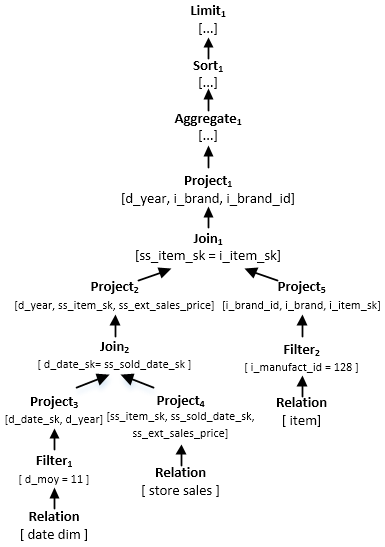
\includegraphics[scale=0.5]{figures/q3}
   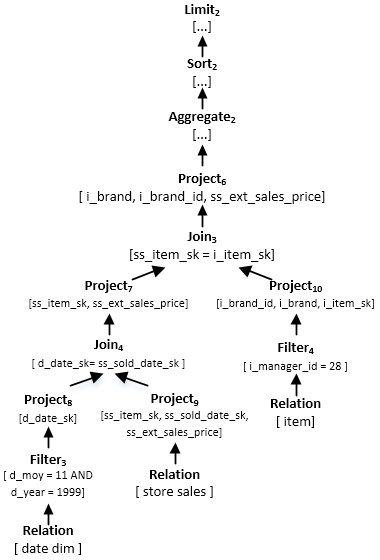
\includegraphics[scale=0.5]{figures/q55}
   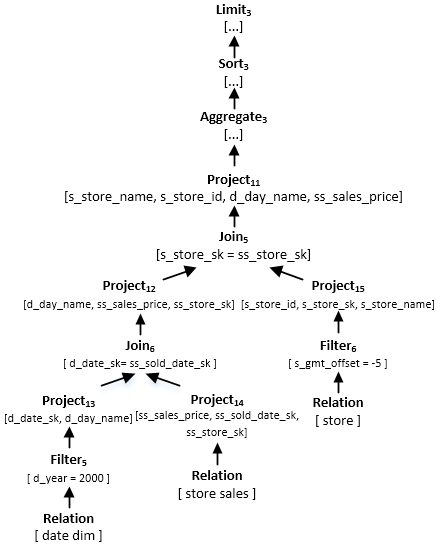
\includegraphics[scale=0.5]{figures/q43}
   \caption{Optimized operator trees of query 3, 55 and 43 (from left to right) in the TPC-DS benchmark} 
   \label{fig:queries}
\end{figure*}

A possibly better sharing option is to let the 3 queries share the greater SEs at ($Project_2$, $Project_7$, $Project_{12}$) so that they will even further benefit from the cost of joining 2 tables \textbf{date dim} and \textbf{store sales}. Furthermore, query 3 and query 55 could share the greatest SEs at ($Project_1$, $Project_6$), joining 3 tables \textbf{date dim}, \textbf{store sales} and \textbf{item}. However, sharing greater SEs is not always better than sharing smaller ones. Specifically in this example, what if the \emph{Join} operator produces a large amount of data that is too expensive to \emph{cache} under a limited amount of memory resource? Note that data caching in memory can be a costly operation, especially in the distributed environment. Our study will show that blindly caching data may lead to higher cost of job execution. One next problem we may have to face is to select multiple CEs that will later become multiple \emph{cache plans} such that the job's performance is maximized while the memory consumption condition is satisfied.

Then, the problem we attempt to solve in this paper can be described as follows: Given a batch of queries submitted, transform it into a more efficient batch such that the new batch results in shorter aggregate job running time, taking into account the memory constraint and extra computations. Particularly in this work, we develop the solution of automatically determining the best cache plans to achieve work sharing for Spark SQL queries. It is the purpose of the following sections to first demonstrate and then evaluate our unified solution for an in-memory cached-based work sharing for large-scale distributed systems.